\documentclass[11pt]{article}

\usepackage{amsmath}
\usepackage{amssymb}
\usepackage[margin=0.68in]{geometry}
\usepackage{booktabs}
\usepackage{enumitem}
\usepackage{fancyhdr}
\usepackage{graphicx}
\usepackage[table]{xcolor}
\usepackage[hidelinks]{hyperref}
\usepackage{listings}
\usepackage{microtype}
\usepackage{tabularx}
\usepackage{titlesec}
\graphicspath{{docs/lessons/assets/}{../assets/}}

\definecolor{Ink}{gray}{0}
\definecolor{CodeGray}{gray}{0.96}
\hypersetup{
  pdftitle={ADK Lesson 030: Inert Show-Cue Simulator},
  pdfauthor={Kevin Shanahan},
  pdfsubject={Synthetic channel assessment, reviewed cue scheduling, deterministic replay, and inert LED evidence},
  pdflang={en-US}
}
\pagestyle{fancy}
\fancyhf{}
\lhead{\textsc{ADK Lesson 030}}
\rhead{Inert Show-Cue Simulator}
\cfoot{\thepage}
\setlength{\headheight}{14pt}
\setlength{\parindent}{0pt}
\setlength{\parskip}{5pt}
\setlist{nosep,leftmargin=1.45em}
\titleformat{\section}{\Large\bfseries\color{Ink}}{\thesection}{0.5em}{}
\titleformat{\subsection}{\large\bfseries\color{Ink}}{\thesubsection}{0.5em}{}
\lstdefinestyle{adkcpp}{
  language=C++,
  backgroundcolor=\color{CodeGray},
  basicstyle=\ttfamily\small,
  keywordstyle=\color{Ink}\bfseries,
  commentstyle=\color{Ink},
  columns=fullflexible,
  keepspaces=true,
  showstringspaces=false,
  frame=single,
  rulecolor=\color{Ink},
  breaklines=true,
  tabsize=4
}
\newcommand{\blank}[1]{\rule{#1}{0.4pt}}
\newcommand{\lessonbox}[1]{%
  \begin{center}\fcolorbox{Ink}{white}{\parbox{0.92\linewidth}{#1}}\end{center}}

\begin{document}

\begin{center}
  {\Huge\bfseries Inert Show-Cue Simulator}\\[4pt]
  {\Large Assess every channel, review every cue, replay every decision}\\[8pt]
  \textit{A composed teaching simulator with no external action path}
\end{center}

\begin{tabularx}{\linewidth}{@{}>{\bfseries}l X >{\bfseries}l X@{}}
Lesson & 030 --- capstone project & Time & 240--300 minutes\\
Prerequisites & Lessons 028 and 029 & Board & Arduino Mega 2560\\
Evidence & TP28, TP29, cue LEDs, RGB state, audit & Status & host verified; bench open\\
Energy class & E1: USB, passive switches, resistor-limited LEDs\\
\end{tabularx}

\lessonbox{\textbf{Boundary.} This project composes synthetic switch
observations with opaque visual cue labels. It has no relay, transistor-driven
load, initiator, show connector, antenna, transmitter, callback, generic output
sink, captured protocol, or external equipment interface. A lit cue is a
teaching-state presentation only. USB power removal is the physical stop;
software cancellation and shutdown are lifecycle behavior, not an emergency
stop.}

\section{Mission and evidence chain}

\[
\begin{split}
\text{eight synthetic observations} &\rightarrow
\text{channel assessment}\\
&\rightarrow\text{reviewed cue decision}
\rightarrow\text{inert LEDs + audit + digest}.
\end{split}
\]

Lesson 028 supplies bounded channel assessments. Lesson 029 supplies a copied
plan, supplied-time scheduler, and append-only audit. Lesson 030 coordinates
their lifecycles and decisions without owning an endpoint or performing I/O.

\subsection{Learning outcomes}

\begin{itemize}
  \item compose two deterministic components through value-only contracts;
  \item map plan positions to channels without interpreting opaque cue IDs;
  \item explain Permit, Hold, and Fault evidence gates;
  \item apply total simultaneous-event precedence;
  \item reconcile snapshots, audit records, and a deterministic trace digest;
  \item distinguish active safe-state evidence from resource-release evidence.
\end{itemize}

\section{Orientation and unpowered inspection}

\begin{center}
% ADK visual: pencil
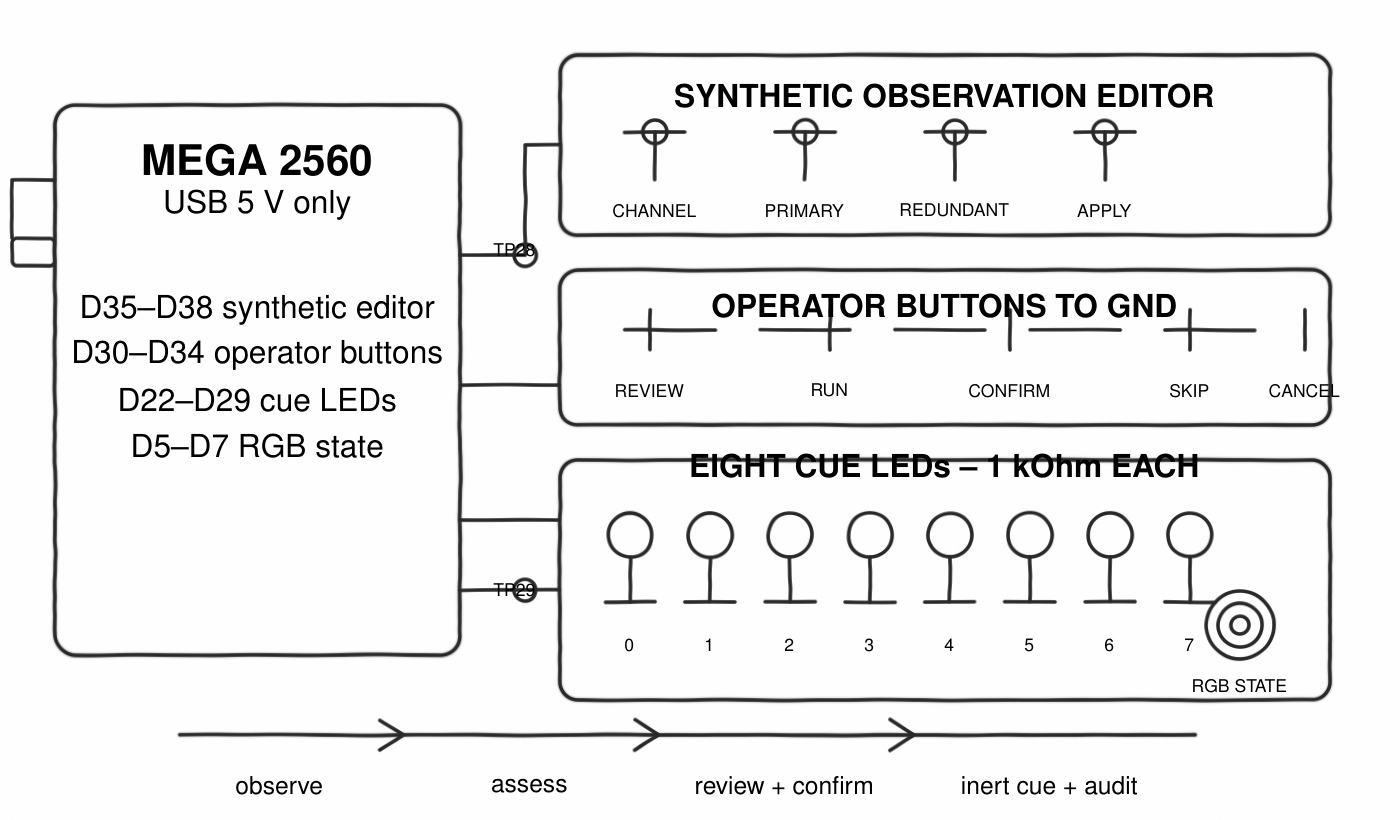
\includegraphics[width=0.96\linewidth]{030-inert-show-pencil.png}

\small\textit{Alternative text: pencil orientation plate showing one
USB-powered Mega, eight synthetic input switches, five pull-up operator
buttons, eight separately resistor-limited cue LEDs, a separately
resistor-limited common-cathode RGB state LED, TP28 at the selected synthetic
input, and TP29 at the selected cue output. No external-load connection is
present.}
\end{center}

\begin{tabularx}{\linewidth}{@{}l l X@{}}
\toprule
Role & Mega pin & Connection\\
\midrule
cue indicators & D22--D29 & pin to 1 k\(\Omega\), LED anode; cathode to GND\\
operator controls & D30--D34 & Review, Run, Confirm, Skip, Cancel to GND; pull-up\\
synthetic editor & D35--D38 & passive switch inputs used to choose test states\\
RGB state & D5--D7 & red, green, blue through separate 1 k\(\Omega\) resistors\\
Lesson 030 TP28 & selected synthetic input & logic-level test point to GND\\
Lesson 030 TP29 & selected cue output & Mega-pin side of resistor to GND\\
\bottomrule
\end{tabularx}

\textbf{Unpowered prediction.} Verify LED polarity, one resistor per LED
channel, switch-to-ground paths, common ground, and no connection outside the
USB-powered fixture. Record resistor values: \blank{1.5in}.

\section{Current, pins, and ownership}

At most one cue channel and one RGB channel are commanded. A conservative
zero-forward-voltage bound gives
\[
I_{\mathrm{channel}}\leq\frac{5.0\ \mathrm{V}}{1000\ \Omega}=5.0\ \mathrm{mA},
\qquad I_{\mathrm{LED,total}}\leq10.0\ \mathrm{mA}.
\]
This is a design calculation, not a measured result.

\begin{tabularx}{\linewidth}{@{}X l l l X@{}}
\toprule
Quantity & Predicted & Measured & Calculated & Interpretation\\
\midrule
USB/5 V rail & at most 5.0 V & \blank{.65in} & --- & \blank{.9in}\\
selected cue resistor & 1 k\(\Omega\) & \blank{.65in} & \(I=(V-V_f)/R\) & \blank{.9in}\\
active RGB resistor & 1 k\(\Omega\) & \blank{.65in} & \(I=(V-V_f)/R\) & \blank{.9in}\\
worst LED load & at most 10 mA & \blank{.65in} & \blank{.75in} & \blank{.9in}\\
\bottomrule
\end{tabularx}

Construction is inert. Initialization starts the assessor, then the scheduler
and its audit session; failure rolls back in reverse order. Shutdown first
forces the scheduler's no-visible-cue state and Shutdown record, then stops the
assessor. The external audit storage deliberately remains readable.

\section{Plan-to-channel composition}

Cue values remain opaque visual labels. The separate map is indexed by plan
position and is copied during construction.

\begin{tabularx}{\linewidth}{@{}r r r r X@{}}
\toprule
Plan index & Cue label & Offset & Visible for & Assessed channel\\
\midrule
0 & 3 & 2000 ms & 2000 ms & 5\\
1 & 7 & 7000 ms & 2000 ms & 2\\
2 & 12 & 12000 ms & 2000 ms & 7\\
3 & 29 & 17000 ms & 2000 ms & 0\\
\bottomrule
\end{tabularx}

\lessonbox{\textbf{Do not infer a channel from a cue.} Cue 3 maps to channel
5, cue 7 maps to channel 2, cue 12 maps to channel 7, and cue 29 maps to
channel 0. The cue LED is addressed with the scheduler's bounded
\texttt{cueIndex}; the selected assessment uses the explicit map.}

The simulator borrows the assessor, scheduler, and audit. Those objects and
their caller-owned storage must outlive it. It allocates no heap storage and
retains no observation pointer.

\section{Complete-frame transaction}

Every accepted update contains exactly eight unique channel observations.
Order does not matter: the simulator canonicalizes them by channel before
identity comparison and digest calculation. Null storage, a wrong count,
duplicate or missing channels, invalid values, and ambiguous time are rejected.

\begin{lstlisting}[style=adkcpp]
const adk::InertShowInput input = {
    observations, 8, operatorInput
};
const adk::Status status = simulator.update(now, input);
const adk::InertShowSnapshot view = simulator.snapshot();
\end{lstlisting}

The pointed-to observations are consumed synchronously; no pointer survives
\texttt{update()}. An identical complete frame repeated at the same timestamp
is idempotent. A changed frame at that timestamp is invalid. The example
samples and decides once per distinct \texttt{millis()} value. It does not
submit a setup-time frame: its first update occurs only after the visible
startup progression, so a same-timestamp button edge cannot be cleared by a
duplicate update.

\subsection{Evidence gate}

\begin{tabularx}{\linewidth}{@{}l l X@{}}
\toprule
Assessment & Gate & Result\\
\midrule
Closed & Permit & confirmation may make the reviewed cue visible\\
Open & Hold & cue stays hidden; wait for a fresh complete frame\\
ShortSimulated & Hold & cue stays hidden with a distinct condition\\
Stale & Hold & cue stays hidden until fresh evidence arrives\\
Unavailable & Hold & cue stays hidden; no automatic bypass\\
Contradictory & Fault & latch fault and guarantee no visible cue\\
\bottomrule
\end{tabularx}

Recovery from a nonterminal Hold never resumes a cue automatically. The
operator returns through review and supplies a fresh confirmation.

\section{State and precedence}

\begin{tabularx}{\linewidth}{@{}l X X@{}}
\toprule
Show state & Meaning & Circuit-native evidence\\
\midrule
Startup & coordinator not active & all cue LEDs inactive\\
Review & operator review gate held & review RGB pattern; cues inactive\\
Ready & waiting or confirming & pending-state RGB pattern; cues inactive\\
Running & scheduler has a visible cue & exactly one cue LED and TP29\\
Held & review or evidence interrupted progress & held RGB; cues inactive\\
Complete & plan ended & completion RGB; cues inactive\\
Cancelled & cancellation latched & cancelled RGB; cues inactive\\
Fault & contradiction, input, invariant, or audit failure & fault RGB; cues inactive\\
\bottomrule
\end{tabularx}

For a newly accepted full frame the total order is:
\[
\boxed{\text{Cancel}\succ\text{invalid chord}\succ
\text{evidence Fault/Hold}\succ\text{Review release}\succ
\text{phase action}\succ\text{time}}
\]
Frame identity is checked first. Cancel therefore wins over simultaneous
Confirm, Skip, or Run, but it does not turn a changed same-timestamp frame into
a second accepted transaction. More than one non-cancel edge is an invalid
chord. Review release prevents confirmation and immediately removes a visible
cue.

\section{Timing and no-catch-up rule}

Run fixes the plan epoch; late decisions never move cue offsets. Confirmation
is accepted only inside its inclusive window. A delayed update records and
hides elapsed work, but does not briefly activate every missed cue. Advancing
from one cue reaches a hidden waiting state first; a later fresh frame assesses
the destination channel before requesting confirmation.

\begin{center}
% ADK visual: pencil
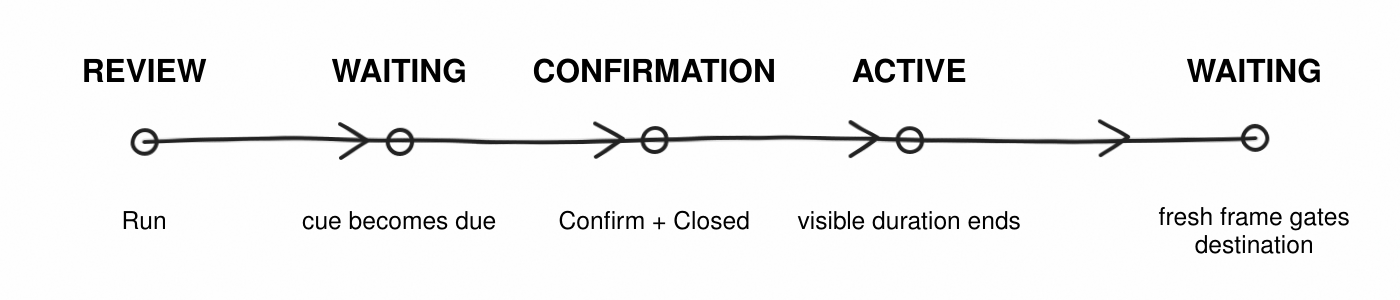
\includegraphics[width=0.96\linewidth]{030-process-pencil.png}

\small\textit{Alternative text: pencil process line from Review through
Waiting, Confirmation, Active, and back to Waiting. Run starts the sequence;
the cue becomes due; Confirm with a Closed assessment begins the visible
interval; its end returns to a destination gate that requires a fresh frame.}
\end{center}

At TP29 predict inactivity before accepted confirmation, a bounded active
interval after it, and immediate inactivity on Hold, Cancel, Fault, completion,
or shutdown. A lit LED proves only the presentation path.

\section{Audit, replay, and digest}

The scheduler remains the sole writer to \texttt{CueAuditBuffer}; the
coordinator does not duplicate records. The ledger never overwrites old
evidence and reserves room for Shutdown before a run begins. If a required
transition cannot be recorded, no corresponding visible transition occurs.

The versioned trace contains supplied ticks, eight synthetic observation
tokens, and debounced operator values. Replay emits stable snapshots; audit
mode emits the stable Lesson 029 audit grammar. The 32-bit trace digest detects
accidental replay differences. It is neither authentication nor a security
control. Repository automation replays the public fixture and checks exact
snapshots and audit records behind the lesson.

\subsection{Trace prediction exercise}

\begin{tabularx}{\linewidth}{@{}l X X X@{}}
\toprule
Frame & Prediction & Observed replay & Reconciliation\\
\midrule
Review + all Closed & \blank{1.05in} & \blank{1.05in} & \blank{1.05in}\\
Run at first epoch & \blank{1.05in} & \blank{1.05in} & \blank{1.05in}\\
Confirm first cue & \blank{1.05in} & \blank{1.05in} & \blank{1.05in}\\
mapped channel Open & \blank{1.05in} & \blank{1.05in} & \blank{1.05in}\\
Cancel + Confirm & \blank{1.05in} & \blank{1.05in} & \blank{1.05in}\\
\bottomrule
\end{tabularx}

For one transition, copy the snapshot sequence \blank{1.0in}, audit sequence
\blank{1.0in}, and final digest \blank{1.1in}. Explain any disagreement:
\blank{2.5in}.

\section{Narrative Mega example}

\begin{lstlisting}[style=adkcpp]
void loop ()
{
    const adk::TimePoint now (millis ());

    observeSimulatorInput (now);
    decideInertShow       (now);
    actuateInertCues      ();
    actuateSimulatorState (now);
}
\end{lstlisting}

Objects appear in dependency order: runtime and claims, buttons, cue and state
LEDs, synthetic source and assessor, plan and audit storage, scheduler, then
simulator. Setup reads as acquire, configure, start. The loop reads as observe,
decide, actuate. Presentation consumes one snapshot and cannot call back into
the simulator. Only after every endpoint and the simulator acquire
successfully does the cue row fill from left to right for two seconds.
Simulator updates begin only after that dependent progression. At two minutes,
an input-independent shutdown makes every output inactive. Serial replay is
optional supporting evidence, never the only observation path.

\section{Predict, observe, interpret}

\begin{enumerate}
  \item Before power, predict TP28 and TP29 outcomes for channel 5 Closed.
  \item Start the fixture. Observe the acquisition sweep separately from the
        later all-cues-inactive safe state.
  \item Hold Review and press Run. Predict TP29 remains inactive before
        confirmation even when the mapped channel is Closed.
  \item Confirm cue 3. Compare the channel-5 TP28 state, selected assessment,
        cue-index-0 LED, TP29, and ordered audit entry.
  \item Make the next mapped channel Open. Predict Hold and no cue; restore
        Closed, renew review, and confirm again.
  \item Inject Contradictory. Predict latched Fault, inactive TP29, and no
        restart until reinitialization.
  \item Let the fixed two-minute session expire without pressing a control.
        Observe immediate darkness; only then remove USB.
\end{enumerate}

\section{Troubleshooting tree}

\begin{tabularx}{\linewidth}{@{}X X@{}}
\toprule
Observation & Stop, inspect, and interpret\\
\midrule
more than one cue LED & remove USB; inspect bounded index presentation\\
wrong cue for TP28 channel & inspect the plan-position map; never use cue ID\\
cue active while Open/Stale & remove USB; inspect gate and fresh-frame logic\\
cue appears before Confirm & remove USB; reject the fixture as valid evidence\\
audit sequence stops & expect AuditFull and no visible transition\\
replay digest differs & compare exact input frames, order, and tool identity\\
out-of-rail TP28 or TP29 & remove USB; inspect ground, switch, and resistor\\
hot part or unstable USB & remove USB immediately; troubleshoot unpowered\\
\bottomrule
\end{tabularx}

\lessonbox{\textbf{Stop rule.} Remove USB power for a hot part, unstable
supply, wrong polarity, missing resistor, unexpected indicator, out-of-rail
TP28 or TP29, or schematic/breadboard disagreement. Do not attach an external
load or real show-control connector. Software shutdown is never the physical
stop.}

\section{Evidence status}

Automated host replay, exception, Mega compilation, measured-size, PDF, and
site checks remain behind this lesson. They do not constitute a physical
result. The repository also retains the formal bench record until a named
board, circuit, instruments, measurements, operator, date, and independent
review are present; the learner is not assigned a command-line workflow or
acceptance card.

\section{Reference trail}

\begin{itemize}
  \item ADK \texttt{inert\_channel\_assessor.h},
        \texttt{inert\_cue\_scheduler.h},
        \texttt{inert\_show\_simulator.h}, focused tests, replay fixture, and
        canonical Lesson 030 sketch;
  \item ADK development, testing, safety, packaging, and PDF policies;
  \item Lessons 028 and 029 for dependency contracts and evidence limits;
  \item Arduino Mega 2560 Rev3 datasheet for the exact board profile.
\end{itemize}

The searchable HTML reference is the primary accessible route. This printable
PDF uses real text, headings, lists, and monochrome graphics but does not claim
PDF/UA conformance.

\end{document}
